%%This is a very basic article template.
%%There is just one section and two subsections.
%\documentclass{article}
\documentclass[a4paper, openany, UTF8, punct, adobefonts]{ctexbook}%{ctexart}
% \documentclass[a4paper, openany, twocolumn, UTF8, punct,adobefonts]{ctexbook}%{ctexart}
% \documentclass[a4paper,twocolumn,12pt]{article}
% \usepackage[top=1in, bottom=1in, left=1.25in, right=1in]{geometry}
% \usepackage[top=1in, bottom=1in, left=1in, right=1in]{geometry}
\usepackage[left={3cm},right={4cm},marginparwidth={3cm},marginparsep={1em},vmargin={2cm},]{geometry}
% \usepackage[top=.6in, bottom=.6in, left=1in, right=1in]{geometry}

% \usepackage{fancyhdr}
% 
% \pagestyle{fancy} \columnsep=10mm
% 
% % \fancyhead[RE]{\leftmark} % 在偶数页的右侧显示章名
% % \fancyhead[LO]{\rightmark} % 在奇数页的左侧显示小节名
% % \fancyhead[LE,RO]{~\thepage~} % 在偶数页的左侧,奇数页的右侧显示页码
% % \fancyfoot[RO,RE]{\it 国防科学技术大学-理学院}
% \renewcommand{\baselinestretch}{1.5}
% \renewcommand{\headrulewidth}{0pt}
% \usepackage[CJKbookmarks=true,bookmarksnumbered,bookmarksopen,colorlinks,linkcolor=blue,anchorcolor=blue,citecolor=green,dvipdfm]{hyperref}
% \excludecomment{student}
% \includecomment{teacher}

\usepackage{amsmath,amsfonts,amssymb,amsthm,bm}
\usepackage{color,graphics,framed}
\usepackage{ulem,enumerate}
% \usepackage{CJKfntef}
\usepackage{esint} %any type of integral symbol
% \usepackage{enumerate}
% \usepackage{esint}

\usepackage{flushend,cuted}

\setCJKmainfont[BoldFont={Adobe Heiti Std}, ItalicFont={Adobe Kaiti Std},
    SlantedFont={Adobe Fangsong Std},
    BoldItalicFont={Adobe Kaiti Std},
    BoldSlantedFont={Adobe Fangsong Std}]{Adobe Song Std}
\punctstyle{CCT}

% \setCJKfamilyfont{zhsong}{Adobe Song Std}
% \setCJKfamilyfont{zhhei}{Adobe Heiti Std}
% \setCJKfamilyfont{zhfs}{Adobe Fangsong Std}
% \setCJKfamilyfont{zhkai}{Adobe Kaiti Std}
% \setCJKfamilyfont{zhli}{LiSu}
% \setCJKfamilyfont{zhyou}{YouYuan}
% 
% \newcommand*{\songti}{\CJKfamily{zhsong}} % 宋体
% \newcommand*{\heiti}{\CJKfamily{zhhei}}   % 黑体
% \newcommand*{\kaishu}{\CJKfamily{zhkai}}  % 楷书
% \newcommand*{\fangsong}{\CJKfamily{zhfs}} % 仿宋
% \newcommand*{\lishu}{\CJKfamily{zhli}}    % 隶书
% \newcommand*{\youyuan}{\CJKfamily{zhyou}} % 幼圆

\renewcommand{\baselinestretch}{1.2}

% %==============std fontspec settings==============
% \usepackage[no-math,cm-default]{fontspec}
% % \newfontfamily\zhfont[BoldFont=Adobe Heiti Std]{Adobe Heiti Std}
% \newfontfamily\zhfont[BoldFont=Adobe Heiti Std]{Adobe Kaiti Std}
% 
% %==============spacing of CH in Xetex==============
% \usepackage{zhspacing} 
% \zhspacing

%==============layout setting==============
\setlength{\parindent}{0pt}  

%===============macros====================
\newcommand{\bb}{\bf\color{blue}}
\newcommand{\ba}[1]{\alert{\bf #1}}
\newcommand*{\e}{\ensuremath{\varepsilon}}
\renewcommand{\b}{\color{blue}}
\newcommand*{\p}{\ensuremath{\partial}}
\newcommand{\limn}{\ensuremath{\lim\limits_{n\to\infty}}}
\newcommand{\sumn}{\ensuremath{\sum\limits_{n=1}^{\infty}}}
\newcommand*{\df}[2]{\displaystyle\frac{\,{#1}\,}{\,{#2}\,}}
\newcommand*{\limx}[1]{\ensuremath{\lim\limits_{x\to{#1}}}}
\newcommand*{\limdx}{\ensuremath{\lim\limits_{\Delta x\to 0}}}
\newcommand*{\dx}{\Delta x}
\newcommand{\dint}{\ensuremath{\displaystyle\int}}
\renewcommand{\d}{\mathrm{d}}
\newcommand{\ds}{\displaystyle}
\newcommand{\ps}[1]{\marginpar{\kaishu\small #1}}

\begin{document}

\definecolor{shadecolor}{rgb}{0.9,0.9,0.9}

% {\kaishu 你好?123}

\section{课程简介}

\subsection{学什么}

\begin{itemize}
	  \item {\bf Wikipedia——微积分} 
	\begin{itemize}
	  \item Latin, {\it a small stone used for counting}  
	  \item {\it a branch of mathematics focused on {\b limits, functions,
	  	derivatives, integrals,}  and {\b infinite series}} 
  	  \item {\it widespread application in {\b science, economics,} and {\b
  	  engineering}} 
% 		  \item {\it constitues a major part of modern mathematics} 
	\end{itemize}
	\item {\bf John von Neumann} ({\small\it The Mathematician, 1947})
	\begin{itemize}
	  \item {\it The calculus was the first achievement of modern
	  mathematics, and it is difficult to overestimate its importance.}
	\end{itemize} 
\end{itemize}

\begin{center}
	\scalebox{0.3}{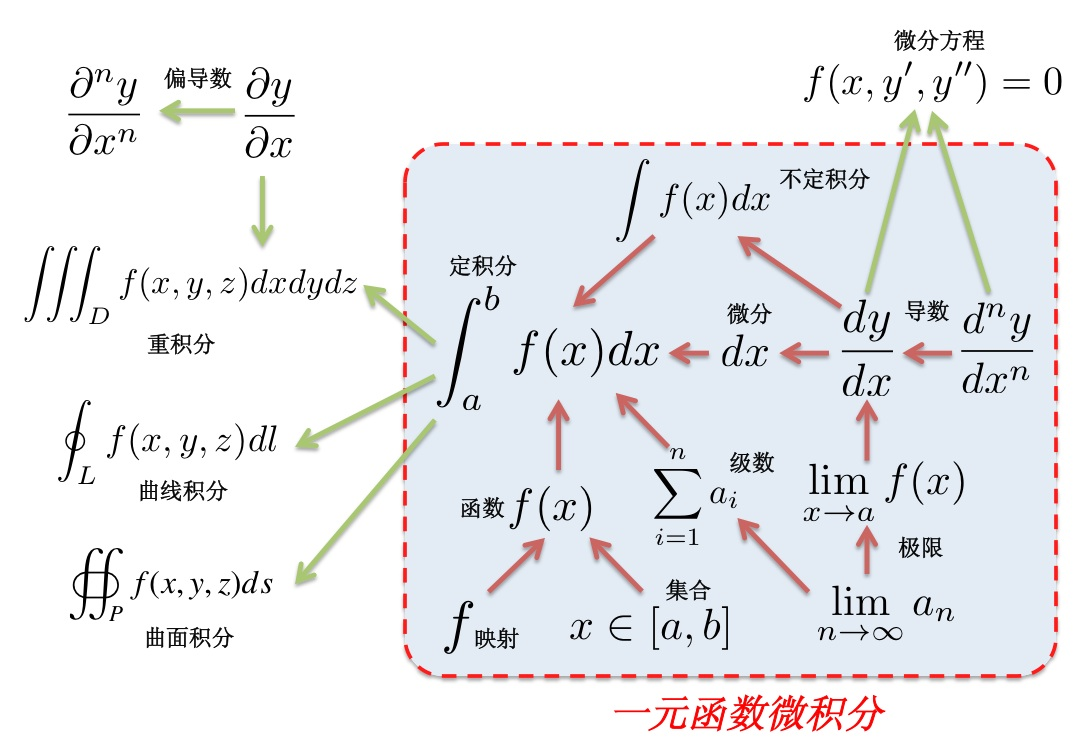
\includegraphics{./images/ch1/AM_architecture.jpg}}
	\ps{上课前画好}
\end{center}

\subsection{怎么学}
	
\begin{itemize}
	\item {\bf 参考资料}
  	\begin{enumerate}
		\item {\bf 课程配套辅导}
	  	\begin{itemize}
	    	\item {李建平 等,高等数学典型例题与解法(上、下),国防科技大学出版社,2009,长沙} 
	  	\end{itemize}
  		\item {\bf 参考书} 
  		\begin{itemize}
	    	\item {\b 同济大学数学系,高等数学(第六版,上、下),高等教育出版社,2006,北京} 
	    	\item 菲赫金哥尔茨,微积分学教程(第一至三卷),第8版,高等教育出版社,2006,北京 
	    	\item James Stewart, Calculus(5th eds.)(影印版,上、下册),高等教育出版社,2004,北京
	    	\item 任何有关教学内容和{\b 数学历史}的书籍
  		\end{itemize}
	\end{enumerate}
	  \item {\bf 学习方法}
	\begin{itemize}
	  		\item {\bf 听课}\dotfill {\bb 30}
		\begin{itemize}
	  		  \item 典型问题、典型方法
	    	  \item 师傅领进门,修行在个人
	 	\end{itemize}
	  		\item {\bf 练习}\dotfill {\bb 50}
	 	\begin{itemize}
	    		\item 熟能生巧!
	    		\item 记忆!琢磨!
	  	\end{itemize}
	  		\item {\bf 思考}\dotfill {\bb 20}
	  	\begin{itemize}
	    		\item 总结!
	    		\item 质疑!
	  	\end{itemize}
	\end{itemize}
\end{itemize}

\section{几点要求}
\begin{itemize}
	\item {\bf 课堂:安静!安静!!安静!!!}
	
	{\bf - No to}
	  \begin{itemize}
	    \item Chatting
	    \item zZZ\ldots
	    \item anything noisy
	    \item \ldots
	  \end{itemize}
	{\bf - Yes to}
  \begin{itemize}
    \item listen to me
    \item discuss {\bf with me}
    \item do sth. you like {\bf quietly}
    \item zzz\ldots
    \item leave/enter the classroom {\bf quietly}
    \item \ldots
  \end{itemize}
  \item {\bf 作业}
  \begin{itemize}
    \item 正确、规范、工整
    \item no copy !!!!
    \item 订正每一个错误!
  \end{itemize}
	\item {\bf 答疑}
	  \begin{itemize}
	    \item 有问必答
	    \item 除了问考试、问隐私
	  \end{itemize}
% 	  \item {\bf 从善如流}
\end{itemize}

\chapter{映射与函数}

{\bf 关键词:}集合、集合论、映射、函数、曲线及其表示

\section{集合与映射}

\subsection{集合}

{\it Cantor,1874:}\ps{对于集合,“我们只需描述它,而不必给出精确的定义”}
所谓{\b 集合},是指把一些个体({\b 元素}) 放在一起考虑时它们形成的整体。
\begin{itemize}
  \item 关系符号:$\subset, \in, =, \subseteq, \neq$
  \item 运算符号:$\cap,\cup, \setminus, \bar{A}, \times, +, - $
\end{itemize}
	
{\bf 常见(用)的集合:}
$\mathbb{N}\subset\mathbb{Z}\subset\mathbb{Q}\subset\mathbb{R}\subset\mathbb{C}$
\ps{本书约定,自然数集包含数$0$}
	
{\bf 注:}通过集合的笛卡尔乘积{\b “$\times$”} 可以定义更{\bf “高维”}的集合,例如:\\
	\centerline{$\mathbb{R}^2=\mathbb{R}\times\mathbb{R}$}

\subsection{区间和邻域}

{\bf 例:}$(a,b)=\{x|a<x<b\}=\{x\in\mathbb{R}|a<x<b\},a,b\in\mathbb{R}$

{\bf 例:}$\mathbb{R}=(+\infty,-\infty)$

{\bf 注意:}$\pm\infty$都不是一个具体的数,因此不能写
$$x=+\infty,\quad x=-\infty$$
而只有
$$x\to+\infty,\quad x\to\infty$$

{\bf 邻域:}“与$a$邻近,距离不超过$\delta$”
$$U(a,\delta)=(a-\delta,a+\delta)=\{x||x-a|<\delta\}$$

{\bf 例:}
$$(a,b)=\left(\df{a+b}2,\df{b-a}2\right)$$

{\bf 去心邻域}
$$U_0(a,\delta)=(a-\delta,a+\delta)-\{a\}=\{x|0<|x-a|<\delta\}$$

{\bf 无穷邻域}
$$\{x||x|>M\},\;M>0$$

{\bf 问:}可以写成$U(\infty,M)$吗?

{\bf 注:}类似地,可以有所谓的半邻域,左(右)邻域

\begin{shaded}

{\bf 集合论、Russell Paradox与公理系统}

	{\it Cantor,1874:}朴素集合论的诞生。	

	{\it Poincare,1900,国际数学家大会:} 
		 {“\ldots 借助集合论概念,我们可以建造整个数学大厦\ldots  今天,我们可以说绝对的严格性已经达到了\ldots”}
	
	{\it Russell, 1901:}只给不给自己理发的人理发的理发师该不该给自己理发?
	
	“由所有不包含集合自身的集合所构成的集合”,记为$S$。不论$S$是不是自身的元素,按照$S$的定义都会有矛盾。
	
	设$x\in A$表示:$A$给$x$理发, 定义
	$$A=\{x|x\notin x\},$$ 
	
	问:$A\in A$还是$A\notin A$? 
	
% 	\ba{罗素悖论导致了第三次“数学危机”的出现!}
	{{\bf {第三次“数学危机”}}(Frege,1901,《算术基础》)}
		“在工作结束之后发现那大厦的基础已经动摇,对于一个科学工作者来说,没有比这更不幸的了”
		
	\begin{itemize}
	  \item {{\bf 无限抽象原则}(Cantor,Frege):} 任意给定某个条件就可以确定一个集合。(每个概念的外延可以确定一个集合)
	  \item {\bf 观点:}不加限制地使用无限抽象原则将导致罗素悖论
	  \item {{\bf 有限抽象原则}(限制公理):} 如果已知一个集合和一个给定的条件,
	  则该集合中所有满足条件的元素{\it 可以}构成一个集合。
	  \item {\bf ZFS(Zermelo-Fraenkel-Skolem)公理化集合系统}
	  
	  {\bf 命题:}在ZFS中,无法定义包含所有集合的集合。
	
	{\bf 证明:}反证法。设$A$是一个这样的集合。定义
	$$B=\{x\in A|x\notin x\}$$
	若
	$B\in A$,则必有$B\in B$或$B\notin B$。而若$B\in B$,可推出$B\notin B$;同理,
	由$B\notin B$,也可推出$B\in B$。从而$B\notin A$,推出矛盾。这说明$B$的定义存在问题,故知假设错误。

	\item {\bf 公理(Axiom):}无须证明即为正确的命题。
	\begin{itemize}
	  \item {\bf Engles:}数学上的所谓公理,是数学需要用作自己出发点的少数思想上的规定 
	  \item {\bf ZFS系统:}公理就是一些关于逻辑符号{“$\in$”}和{字母}的组合使用方法的约定
	  \item {\bf 公理化方法}是构建现代数学理论体系的基石
	\end{itemize}
	\item {\bf {数学等于永恒的真理吗?}}
	\end{itemize}
\end{shaded}
	
\subsection{实数集的性质}
	\begin{enumerate} 
	  \item {\bf 有序性}($\mathbb{R}^2$、$\mathbb{C}$不具备有序性) 
	  \ps{$\mathbb{R}$是全序的,而$\mathbb{R}^2$、$\mathbb{C}$在一定的度量下
	  是半序的}
	  \item {\bf 完备性(连续性): }实数集与数轴上的点之间存在一一对应
	  
	  {\bf{连续性公理(确界原理):}}非空有{上界}的实数集必有{上确界} (最小的上界)
	\end{enumerate}
	
	{\bf 注:}有理数集不满足连续性公理。
	\ps{有理数集的有限次四则运算仍是有理数}
	
	{\bf 例:$e=\mathrm{sup}\left\{\left(1+\frac
	1n\right)^n\right|n\in\mathbb{N}\}\notin\mathbb{Q}$}
	\begin{center}
		\resizebox{!}{5cm}{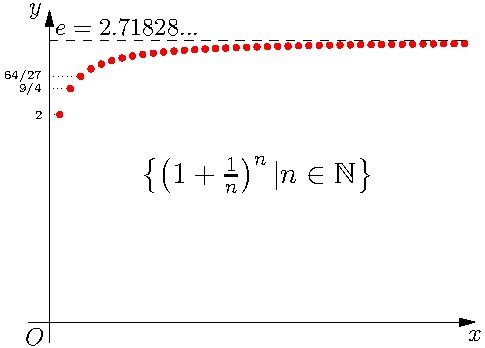
\includegraphics{./images/ch1/e-notin-N.pdf}}
% 		\resizebox{!}{4.8cm}{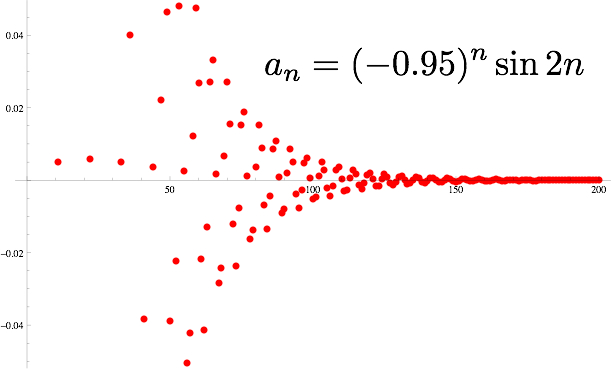
\includegraphics{./images/ch2/sin2nn.jpg}}
% 		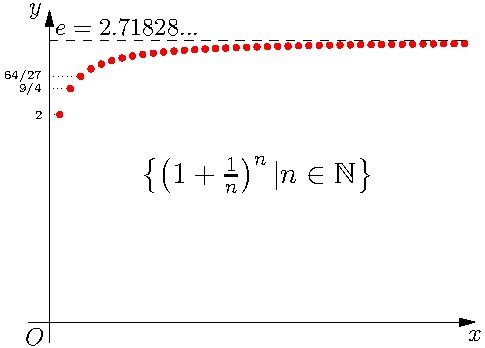
\includegraphics[width=6cm]{./images/ch1/e-notin-N}
	\end{center}
	$$\left(1+\frac11\right)^1<\left(1+\frac12\right)^2<\left(1+\frac13\right)^3<\ldots
	\left(1+\frac1n\right)^n<\ldots<e$$
	
	{\bf 思考:}上确界和最大值有什么异同?如何确定一个集合的上确界?

\subsection{映射}

{\bf 教材P7:}事物之间“一对一”或“多对一”的依赖关系\ps{映射结果必须是无歧义的!}

$$f:A\to B$$
或
$$y=f(x),\;x\in A,y\in B$$

{\bf 三要素:}定义域、值域、对应关系,任何一项不明确都不足以确定一个函数
\ps{有时候只有定义域和对应关系亦可,前提是默认假设映射为满射}

{{\bf 例:}以下函数中哪些是完全相同的?}
		$$x,\quad |x|,\quad e^{\ln x},\quad \ln(e^x),\quad \sqrt{x^2},\quad
		\frac{x^2-4}{x-2}-2,$$
		$$\sin(\arcsin x),\quad \arcsin(\sin x), \quad \tan(\arctan x)$$

{\bf 相关概念:}单射、满射、一一映射(双射)

\begin{shaded}
	{\bf 一一映射与无穷集合}
	
{\bf 问题:}如何比较两个集合中元素的个数?
\begin{itemize}
  \setlength{\itemindent}{1cm}
  \item 自然数与正偶数“一样多”?({$\surd$})
  \item 自然数与整数“一样多”?({$\surd$})
  \item 自然数与有理数“一样多”?({$\surd$})
  \item 区间$(a,b)$中的实数与$\mathbb{R}$中“一样多”?({$\surd$})
  \item 自然数与实数“一样多”?({$\times$})
\end{itemize}
	
{\bf 无穷集合:}可以和自身的某个子集建立起一一映射的集合
\end{shaded}	

	
\section{函数}
	
	\begin{shaded}
		{\bf 关于函数}
		\begin{itemize}
  		  \setlength{\itemindent}{1cm}
		  \item 微积分是关于运动和变化的数学;
		  \item 函数是对运动(例如:曲线、曲面、波以及各种变化)变化过程中各种量与量的依赖关系的抽象描述;
		  \item 函数刻画了运动变化中的量之间的相互依存关系({\bf 注:}与“依存”对应的关系叫做“独立”)
		\end{itemize}
		
		{\bf 常量和变量}
		\begin{itemize}
  		  \setlength{\itemindent}{1cm}
		  \item {\bf 常量和变量是相对的},在一定条件下可以相互转化
		  \item 变量之间的关系可能是相互依存,也可能是相互独立的
		  \item 为了避免讨论过于复杂,简化问题,我们可能选择只考虑部分参数的变化,而将其他参数视为(或设为)常量,
		  例如:万有引力与两个物体的质量、距离以及引力常数(系数)都有关,为了确定其数量关系,需要事先假定部分的参数
		  值是固定不变的
		\end{itemize}
		
		{\bf 大学数学与中学数学}
		\begin{itemize}
  		  \setlength{\itemindent}{1cm}
		  \item 数学并无严格的“高等”和“初等”之分,只是存在众多的分支和领域
		  (例如:代数、几何、分析、图论,几何又分为平面几何、立体几何、解析几何等),
		  不同分支或领域的直观性和难度各有不同
		  \item 对于函数,中学阶段更注重在对应关系“确定”的情况下,寻找其数学描述或利用给定的值进行计算
		  \item 大学阶段,从微积分开始,更着重对函数的整体特性,以及不同函数间的转换、类比和关于其整体特征的计算与分析
		\end{itemize}
		
		 {\bf James Stewart, Calculus(5th eds.), 2004}
		  \begin{itemize}
  		    \setlength{\itemindent}{1cm}
		    \item {\it Calculus is fundamentally different from the mathematics that
		    you have studied previously}
		    \item {\it Calculus is less static and more {\b dynamic}}
		    \item {\it It is concerned with change and {\b motion}}
		    \item {\it It deals with quantities that {\b approach} other
		    quantities}%\marginpar{note}
		  \end{itemize}
	\end{shaded}

	{\bf (一元)函数:}由实数集到实数集的映射
	$$f:D\to\mathbb{R},\;(D\subset\mathbb{R})$$
	或
	$$y=f(x),\;(x\in D\subset\mathbb{R},y\in\mathbb{R})$$
% 	\begin{itemize}
% 	  \item {\bf 定义域:} $D\subset \mathbb{R}$ ,且$D\ne\phi$ 
% 	  \item {\bf 对应关系:} $f:D\to\mathbb{R}$
% 	\end{itemize} 
	{\bf 函数图像}
	$$G_f=\{(x,f(x))|x\in D_f\}$$
	
	\begin{shaded}
		{\bf 多元函数:} 
		$$f:D\to\mathbb{R},\quad D\in\mathbb{R}^n$$
		
		{\bf 向量值函数:}
		$$f:D\to\mathbb{R}^,\quad, D\in\mathbb{R}$$
		
		{\bf 思考:}二元函数和三维的向量值函数对应的几何对象分别是什么?
		
		{\bf 思考:}平面曲线与一元函数具有一一对应关系吗?空间曲面和二元函数呢? (No)	
	\end{shaded}	
		\begin{center}
			\resizebox{!}{4.2cm}{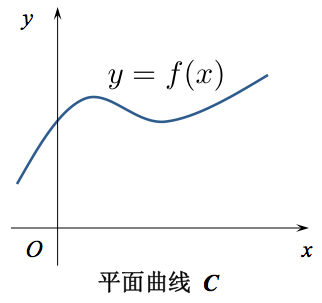
\includegraphics{./images/ch1/C_fx.jpg}}\quad	
			\resizebox{!}{4.5cm}{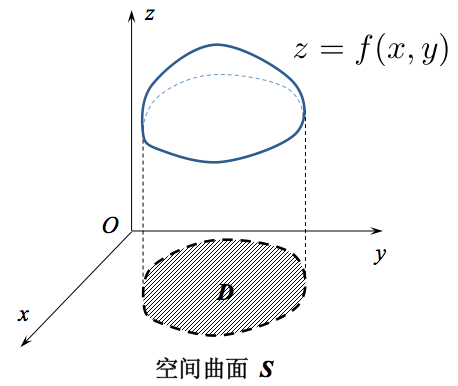
\includegraphics{./images/ch1/S_fxy.jpg}}
		\end{center}
	
\subsection{函数的运算与简单性质}

{\bf 运算:}四则运算、复合运算、逆运算	
	
\begin{shaded}
{\bf 常用数学符号}
	\begin{itemize}
	  \item {$\bm{\forall}$} \quad 任意 (for all)
	  \item {$\bm{\exists}$} \quad 存在 (exist)
	  \item {$\bm{\Rightarrow}$} \quad 推出 (deduce, imply)
	  \item {$\bm{\Leftrightarrow}$} \quad 等价 (equivalent, if and only if)
	  \item {$\bm{\to}$} \quad 趋于 (approach)
	\end{itemize}
\end{shaded}

\subsubsection{【有界性】}			

{{\bf 定义:}}
	设$I\subset\mathbb{R}$,$f(x)$在$I$上有定义,若集合
	$$\{f(x)|x\in I\}$$
	有界,则称{\bf $f(x)$在$I$上有界}或{\bf $f(x)$是$I$上的有界函数}
		
	{\bf 注:}函数的有界性等价于其值域的有界性

	{{\bf 例:}指出如下函数的有界性}
	
		\quad(1)\;$y=\arctan x$,\hspace{2em} (2)\;$y=e^x$,\hspace{2em}
		(3)\;$y=x\sin x$
		
\begin{shaded}
	{\bf “反面定义”(否命题)的写法*}
	\begin{enumerate}
	  \item {“任意”和“存在”互换}
	  \item {“$\geq(\leq)$”和“$<(>)$”互换}
	\end{enumerate}
	
	【提示】:参考De Morgen律,任何命题的成立都是与一定范围有关的
	
	{\bf 定义'}(无界性)
		设函数$f:D\to\mathbb{R}$,若对$\forall M$,$\exists x_M\in D$,使得
		$f(x_M)>M$,则称{\bf $f(x)$无上界}。

\end{shaded}		

\subsubsection{【单调性】}

{{\bf 定义:}}设$f:I\to\mathbb{R}$,若$\forall x_1,x_2\in I$
$$x_1<x_2\Rightarrow f(x_1)\leq f(x_2)$$
则称{\bf $f(x)$在$I$上单调递增}(若不等式中的等号总是无法成立,则称其为严格单调递增)
	
{{\bf 例:}讨论如下函数的单调性}

	\quad(1)\;$y=x\mathrm{sgn}(x)$\hspace{3cm}(2)\;$y=x+\sin x$

{\bf 注:}严格单调的函数一定存在反函数。反之呢?\ps{要说明一个命题不成立,只需举出反例即可}

\subsubsection{【奇偶性】}

{{\bf 定义:}}
	设函数$f:\mathbb{R}\to\mathbb{R}$,
	{\bb 称$f(x)$为偶函数},是指: 对$\forall x\in\mathbb{R}$,有
	$$f(-x)=f(x)$$

{{\bf 例:}试给出如下性质的数学定义}
\begin{enumerate}[(1)]
  \setlength{\itemindent}{1cm}
  \item 函数$y=f(x)$的图像关于$x=a$对称
  \item 函数$y=f(x)$的图像关于点$(x_0,y_0)$对称
\end{enumerate}

{{\bf 思考:}$f(x)=g(a-x),\;(x\in\mathbb{R})$有什么几何意义?}

【提示】:$\sin(x)=\cos(\pi/2-x)$

\subsubsection{【周期性】}

{{\bf 定义:}}
设函数$f:\mathbb{R}\to\mathbb{R}$,
称{\bb $f(x)$为周期函数},是指: $\exists T>0$,
使对$\forall x\in\mathbb{R}$,有
$$f(x+T)=f(x).$$
 满足以上性质的最小正数$T$称为$f(x)$的{\bb 最小正周期}
		 
{\bf 注:}若$T$为$f(x)$的一个周期,$n\in\mathbb{Z}$,则$\forall x\in\mathbb{R}$
$$f(x+nT)=f(x)$$

\subsection{常用函数}

\subsubsection{\bf 【符号函数】}

  $$\bm{\mathrm{sgn}}\,x =\left\{
	\begin{array}{rl}
	-1,\;&x<0 \\
	0,\;&x=0 \\
	1,\;&x>0
	\end{array}
  \right.$$
  {\bf 注:}$|x|=x \cdot\mathrm{sgn} x$
	

 \subsubsection{\bf 【取整函数】}

  $$y=\left[ \,x\, \right]$$
  $[\,x\,]$表示小于等于$x$的最大整数

	
{\bf 注:}有时候还有所谓的上取整和下取整函数

{{\bf 例:}给出以下曲线的方程}

\begin{center}
	\resizebox{!}{2.5cm}{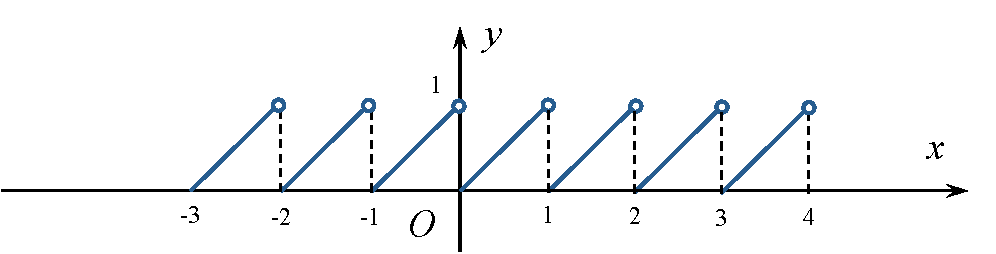
\includegraphics{./images/ch1/f1.pdf}}\quad $x-[x]$\\

	\resizebox{!}{2.5cm}{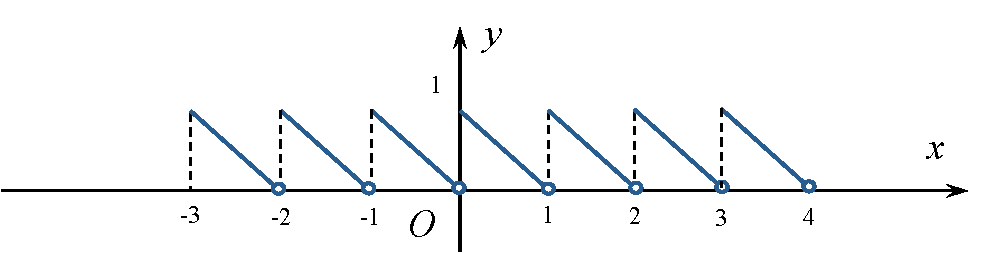
\includegraphics{./images/ch1/f2.pdf}}\quad $[x]-x+1$\\

	\resizebox{!}{2.5cm}{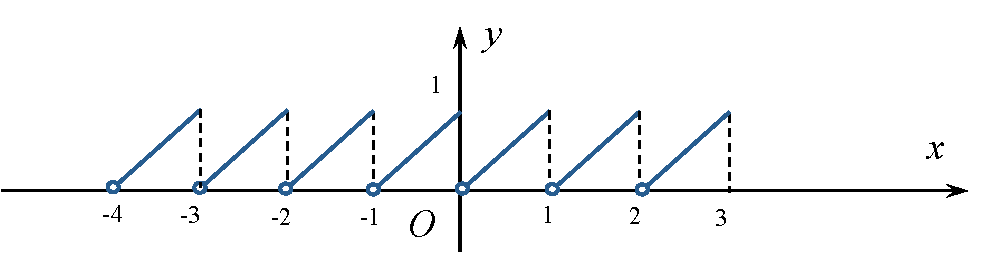
\includegraphics{./images/ch1/f3.pdf}}\quad $[-x]+x-1$
\end{center}
	
{\bf 例:}$(-1)^{[x]}$的图像?方波!

\subsubsection{\bf 【Dirichlet函数】}
  $$\bm{D}(x) =\left\{
  \begin{array}{ll}
  	1,\;& x\in\mathbb{Q} \\
  	0,\;& x\notin\mathbb{Q}
  \end{array}
  \right.$$
  \begin{itemize}
    \item $D(x)$在实数轴上处处无极限
	\item $D(x)$在实数轴上处处不连续
	\item {\b 仅在一点连续的函数:}$xD(x)$
  \end{itemize}

\subsubsection{\bf 【Riemann函数】*:} 

$(x\in[0,1])$
  $$\bm{R}(x) =\left\{
	\begin{array}{ll}
	1,\;&x=0\\
	\displaystyle\frac 1q,\;&x=\displaystyle\frac pq,\,p,q\mbox{互素}\\
	0,\;&x\notin\mathbb{Q}
	\end{array}
  \right. $$
  \begin{itemize}
    \item 对任意$x_0\in[0,1]$, $\lim\limits_{x\to x_0}R(x)=0$
    \vspace{1ex}
    \item $R(x)$在{\b 无理数点连续, 有理数点不连续}
  \end{itemize}

\subsubsection{【初等函数】}

\begin{enumerate}
  \item {\bf 幂函数:} $y=x^a,\; (a\in\mathbb{R})$\ps{只有整数次幂的函数可以手工计算!!!}
  \item {\bf 指数函数:} $y=a^x,\; (a>0,a\ne 1)$
  \begin{itemize}
    \item {\b $y=e^x$}
  \end{itemize}
  \item {\bf 对数函数:} $y=\log_ax,\; (a>0,a\ne 1)$
  \begin{itemize}
    \item {\b$y=\ln x$}
  \end{itemize}
  \item {\bf 三角函数:} $\sin x, \,\cos x,\, \tan x, \,\cot
  x,\, \sec x,\, \csc x$
  \item {\bf 反三角函数:} $\arcsin x, \,\arccos x, \arctan x,
  \ldots$
\end{enumerate}
{\bf{要求:}} 熟练掌握初等函数的定义、性质和相互推导的公式


\subsubsection{【($n$)次多项式(函数)】}

  $$P_n(x)=\sum_{i=0}^na_ix^i,
  \;(a_i\in\mathbb{R},i=1,2,\ldots,n)$$
  \begin{itemize}
    \item { $n$次多项式方程$P_n(x)=0$在$\mathbb{R}$上最多有$n$个根 (包含重根) ,在
    $\mathbb{C}$上有且仅有$n$个根(包含重根)}
    \item { 设$x_i\in\mathbb{C}(i=1,2,\ldots,n)$为$P_n(x)=0$的全部根 ,则
    $$P_n(x)=a_n\prod_{i=1}^n(x-x_i)$$}
    \item { 已知$P_n(x)$在$n+1$个点处的值, 可以唯一确定$P_n(x)$}
  \end{itemize}

\subsubsection{【有理函数】}

$$f(x)=\frac{P(x)}{Q(x)}, \quad\mbox{其中}P(x),Q(x)\mbox{均为多项式函数}$$
  
{\bf 注:}任意有理函数总可以化为一个多项式函数和一个真分式(分子的次数比分母低的有理函数)
的和
	  
{{\bf 例:}用多项式除法化简以下函数}
$$\frac{5x^3+3x^2+1}{x+1}$$

\subsubsection{【双曲函数】}

{\small $$\sinh x =\df{e^x-e^{-x}}{2}, \quad
\cosh x =\df{e^x+e^{-x}}{2}, \quad\tanh x=\df{\sinh
x}{\cosh x}, \ldots$$}

\section{曲线的参数方程和极坐标方程}

{\bf 问题:}$y=f(x)$能否表示平面上的所有曲线?
	
{\bf 或者:}怎样才能更好地表示平面上的曲线?\ps{例如:$x^2+y^2=1,xy=1,x=y^2,\ldots$}

\begin{shaded}
	\begin{center}
		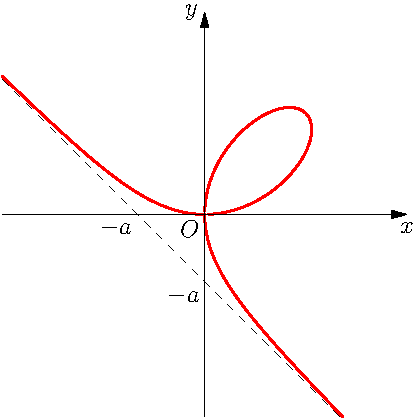
\includegraphics[width=5.5cm]{./images/ch1/dicartesCurve.pdf}

		{\bf Descartes叶形线}
	\end{center}
	\bigskip
	\begin{itemize}
	  \item {\bf 参数方程:}
	  	$$\left\{\begin{array}{l}
	  		x=\df{3at}{1+t^3},\\[1em] y=\df{3at^2}{1+t^3}
	  	\end{array}\right.\;(t\in\mathbb{R})$$
	  	\vspace{-1em}
	  \item {\bf 隐函数方程:}
	  	$$x^3+y^3-3axy=0$$
	\end{itemize}
\end{shaded}

{\bf 例:}求过平面上两点$P_i(x_i,y_i)\,(i=1,2)$的直线方程
		  
$$k=\df{y_2-y_1}{x_2-x_1}=\df{y_2-y_1}{x_2-x_1}$$
由此可给出直线的平面直角方程。若参数化
$$\df{y_2-y_1}{y_2-y_1}=\df{x_2-x_1}{x_2-x_1}=t$$
则有
$$y=ty_2+(1-t)y_1,\quad x=tx_2+(1-t)x_1,\quad (t\in\mathbb{R})$$
		  
{\bf 注:}
\begin{itemize}
  \setlength{\itemindent}{1cm}
  \item 参数方程必须标明参数的取值范围!!!
  \item {利用参数方程可以表示平面上的任意曲线}
  \item {任意曲线的参数方程均不唯一}
\end{itemize}

\subsubsection{【极坐标】}

$$(x,y)\;\to\;(\rho\cos\theta,\rho\sin\theta)\quad
(\rho>0,\theta\in\mathbb{R})$$
	
{{\bf 例:}求以下曲线的极坐标方程\hfill P38-例9}
		
\begin{enumerate}[(1)]
  \setlength{\itemindent}{1cm}
  \item $y=kx,(k\in\mathbb{R})$
  \item $x+y=1$
  \item $x^2+y^2=R^2,\,(R>0)$
  \item $(x^2+y^2)^2=2a^2xy$
\end{enumerate}
	
{\bf 思考:}将极坐标方程化为平面直角方程应注意些什么?

\newpage

\section*{课后作业}
	
\begin{itemize}
  \item 习题1.1:4(2),10
  \item 给出P9例6中二维球极投影映射中:
  
  (1)$Q$的极坐标与$P$的横坐标的对应关系;
  
  (2)$Q$的坐标与$P$的坐标的对应关系;
  
  (3)描述如何将一个单位球面映射为一个二维平面,给出相应的坐标对应关系。
  \item 习题1.2:8,12,13,21
  \item 给出P23例14中的三角波的函数表达式
  \item 习题1.3:5
\end{itemize}

{\bf 【课堂练习与思考题】}

\begin{itemize}
  \item 习题1.1:(C)应用题
  \item 习题1.2:3,17
  \item 习题1.3:6
  \item 阅读:李开复,《给未来的你》
\end{itemize}

\newpage

\section*{参考解答}

1. 习题1.1:10,证明:
$$\df{a_1+a_2+\cdots+a_n}n\geq\sqrt[n]{a_1a_2\cdots a_n},$$
其中$a_i(i=1,2,\ldots,n)$均为非负实数。

证法一:易证$n=2$时不等式成立。假设对$n=2^k(k\in\mathbb{Z}_+)$不等式成立,则
当$n=2^{k+1}$时,
\begin{eqnarray*}
	a_1+a_2+\cdots+a_{2^{k+1}}&\leq&2^k\sqrt[2^k]{a_1a_2\cdots a_{2^k}}
	+2^k\sqrt[2^k]{a_{2^k+1}+a_{2^k+2}+\cdots+a_{2^{k+1}}}\\
	&\geq&2\cdot 2^k\sqrt{\sqrt[2^k]{a_1a_2\cdots a_{2^k}}\cdot
	\sqrt[2^k]{a_{2^k+1}+a_{2^k+2}+\cdots+a_{2^{k+1}}}}\\
	&=&2^{k+1}\sqrt[2^{k+1}]{a_1a_2\cdots a_{2^{k+1}}}
\end{eqnarray*}
由数学归纳法,可知当$n$取$2$的整数次幂时,不等式成立。

若$n$不等于$2$
的某个整数次幂,不妨设$2^{k-1}<n<2^k(k\in\mathbb{N})$,于是
\begin{eqnarray*}
	& &a_1+a_2+\cdots+a_n+\left(2^k-n\right)\sqrt[n]{a_1a_2\cdots a_n}\\
	& & \quad\geq 2^k\sqrt[2^k]{a_1a_2\cdots a_n\left(\sqrt[n]{a_1a_2\cdots
	a_n}\right)^{2^k-n}}\\
	& &\quad =2^k\sqrt[n]{a_1a_2\cdots a_n}
\end{eqnarray*}
以上不等式稍加整理即证。

证法二:易证$n=2$时不等式成立。以下假设$n=k$时不等式也成立,即
$$\df{a_1+a_2+\cdots+a_k}{k}\geq\sqrt[k]{a_1a_2\cdots a_k}.$$
当$n=k+1$时,记$t=a_1+a_2+\cdots+a_k$,且不妨设$a_{k+1}=\max\{a_1,a_2,
\cdots,a_{k+1}\}$,即$ka_{k+1}\geq t$,也是
\begin{eqnarray*}
	\left(\df{a_1+a_2+\cdots+a_{k+1}}{k+1}\right)^{k+1}
	&=&\left(\df{t+a_{k+1}}{k+1}\right)^{k+1}
	=\left[\df tk+\df{ka_{k+1}-t}{k(k+1)}\right]^{k+1}\\
	&\geq&C_{k+1}^0\left(\df tk\right)^{k+1}+C_{k+1}^1\left(\df tk\right)^k
	\df{ka_{k+1}-t}{k(k+1)}\\
	&=&\left(\df tk\right)^ka_{k+1}\geq a_1a_2\cdots a_{k+1}
\end{eqnarray*}
即证。
\bigskip

2.给出P9例6中二维球极投影映射中:
  
(1)$Q$的极坐标与$P$的横坐标的对应关系;
  
(2)$Q$的坐标与$P$的坐标的对应关系;
  
(3)描述如何将一个单位球面映射为一个二维平面,给出相应的坐标对应关系。

解:
\begin{center}
	\resizebox{!}{5cm}{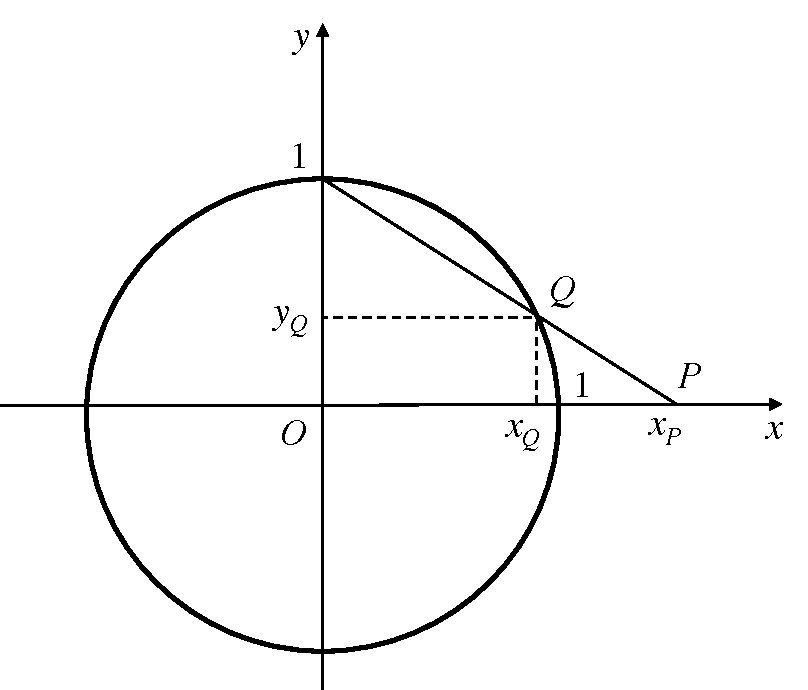
\includegraphics{./images/ch1/answer/sphereline2D.pdf}}\quad
	\resizebox{!}{5cm}{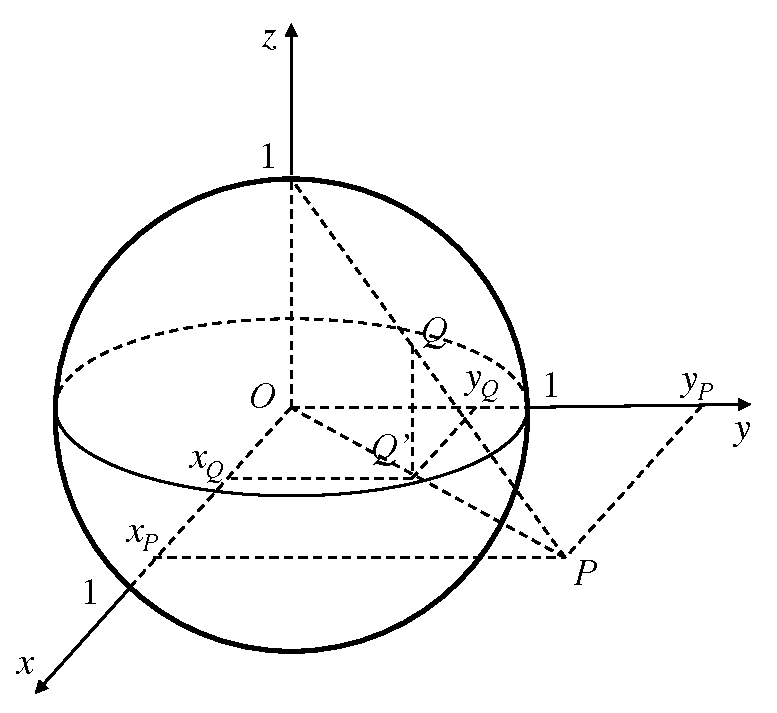
\includegraphics{./images/ch1/answer/sphereline3D.pdf}}
\end{center}
(1)(2) 如左图,设$P,Q$的坐标分别$(x_P,0),(x_Q,y_Q)$,则有
$$
\left\{
\begin{array}{l}
	x^2_Q+y^2_Q=1\\
	\df{x_Q}{x_P}+y_Q=1
\end{array}
\right.
$$
由此可解得
$$y_Q=\df{1-x^2_P}{1+x^2_P},\quad x_Q=\df{2x_P^3}{1+x^2_P}.$$
进而可知$Q$的极坐标为$(1,\theta)$,其中
$$\theta=
\left\{
\begin{array}{ll}
	\arctan\df{1-x^2_P}{2x^3_P},& x_P>0\\
	\pi+\arctan\df{1-x^2_P}{2x^3_P}, & x_P<0
\end{array}
\right.
$$
(3)如右图,设$P,Q$的坐标分别$(x_P,y_P,0),(x_Q,y_Q,z_Q)$,则有
$$
\left\{
\begin{array}{l}
	x^2_Q+y^2_Q+z^2_Q=1\\
	\df{x_Q}{x_P}=\df{y_Q}{y_P}=1-z_Q
\end{array}
\right.
$$
由此可解得
$$
\left\{
\begin{array}{l}
	x_Q=\df{2x_P(x^2_P+y^2_P)}{1+x^2_P+y^2_P}\\
	y_Q=\df{2y_P(x^2_P+y^2_P)}{1+x^2_P+y^2_P}\\
	z_Q=\df{1-x^2_P-y^2_P}{1+x^2_P+y^2_P}
\end{array}
\right.
$$

\bigskip

3.习题1.2:8,题略

\begin{center}
	\resizebox{!}{6cm}{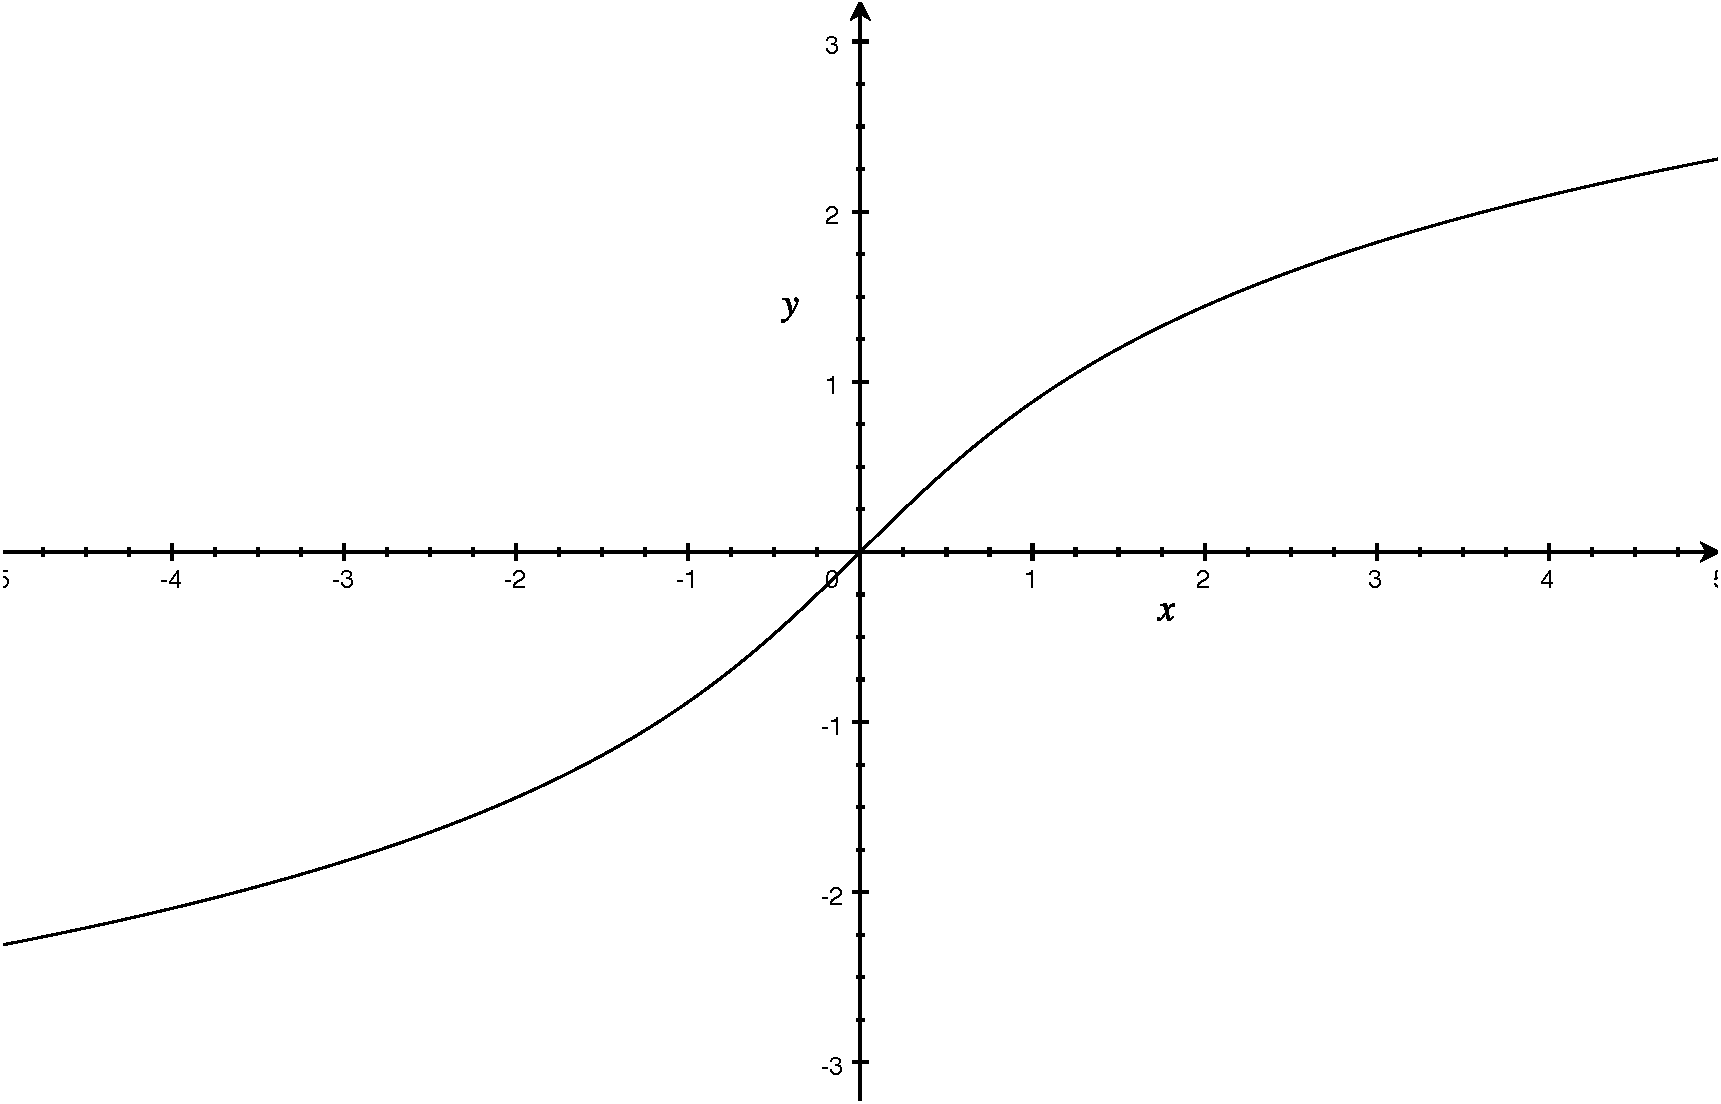
\includegraphics{./images/ch1/answer/lx.pdf}}
	
	$y=\ln(x+\sqrt{1+x^2})$的函数图像
\end{center}

\bigskip

4.习题1.2:17,题略

参考答案:
$$f_c(x)=\df12\left(|f(x)+C|-|f(x)-C|\right)$$

\bigskip

5. 习题5.2:3,证明恒等式

(1)$3\arccos x-\arccos(3x-4x^3)=\pi,\left(|x|\leq\df12\right)$

(2)$2\arctan x+\arcsin\df{2x}{1+x^2}=\pi,(x>1)$

证:(1)注意到
$$\cos(3\arccos x)=4[\cos(\arccos x)]^3-3\cos(\arccos
x)=4x^3-3x=\cos[\pi-\arccos(3x-4x^3)].$$
由此可知
$$3\arccos x=2k\pi-\pi+\arccos(3x-4x^3)\quad(k\in\mathbb{Z}).$$
又当$|x|\leq\df12$时,$|3x-4x^3|\leq 1$,进而
$$\pi+\arccos(3x-4x^3)\in[\pi,2\pi],\quad 3\arccos x\in[\pi,2\pi].$$
从而可知必有
$$3\arccos x=\pi+\arccos(3x-4x^3),$$
即证。

(2)由于
$$\sin(2\arctan x)=\df{2\tan(\arctan x)}{1+\tan^2(\arctan
x)}=\df{2x}{1+x^2}=\sin\left(\pi-\arcsin\df{2x}{1+x^2}\right)$$
从而可知
$$2\arctan x=2k\pi+\pi-\arcsin\df{2x}{1+x^2}\quad(k\in\mathbb{Z}).$$
又当$x>1$时,$2\arctan x\in\left(\df{\pi}2,\pi\right),\df{2x}{1+x^2}\in(0,1)$,进而
$$\pi-\arcsin\df{2x}{1+x^2}\in\left(\df{\pi}2,\pi\right),$$
由此可知必有
$$2\arctan x=\pi-\arcsin\df{2x}{1+x^2},$$
即证。

% \setcounter{chapter}{1}

\chapter{数列极限与数值级数}

\section{数列极限}

\subsection{数列}

{\bf 教材P45:}按一定规律排列的无穷多个(相同或不相同的)数,记作:
$$a_1,a_2,\ldots,a_n,\ldots$$
或者$\{a_n\}$。

$\{a_n\}$的实质是定义在$\mathbb{N}_+$上的函数,即所谓的{\bf 整标函数}\ps{教材上的说法是“可视为”},即
$$a_n:\mathbb{N}_+\to\mathbb{R}$$

{\bf 命题:}一个集合是可数的,当且仅当它可以表示为一个数列。

{\bf 思考:}数列与集合有哪些区别?\ps{1、有序-无序;2、无限-可能有限;3、可重复-不可重复}

{\bf 例:}数列举例

\begin{enumerate}[(1)]
  \setlength{\itemindent}{1cm}
  \item[(1)] $\left\{\df{n+1}n\right\}:\df 21,\df 32,\df43,\df54,\df65,\ldots$
  \item[(2)] $\left\{\df{(-1)^n}n\right\}:-1,\df12,-\df13,\df14,-\df15,\df16,\ldots$
  \item[(3)] $\{n^2\}:1,4,9,16,25,36,\ldots$
  \item[(4)] $\left\{n^{(-1)^n}\right\}:1,2,\df13,4,\df15,6,\ldots$
\end{enumerate}

\subsection{数列的极限}

{\bf 极限:} 一种无限靠近的趋势 
	
\begin{enumerate}
  \setlength{\itemindent}{1cm}
  \item 对于数列而言,无限靠近的趋势意味着什么? 
  \item 如何从数学上严格表达这种趋势? 
\end{enumerate}

{\bf 定义2.1.2} 

对于数列$\{a_n\}$,若存在常数$a$,对于任意给定的正数$\e$,均存在正整数$N$,当$n>N$时,恒有
$$|a_n-a|<\e$$
成立,则称{\bf 数列$\{a_n\}$存在极限(或收敛)},常数$a$称为该数列的极限,记为
$$\lim_{n\to\infty}a_n=a$$
或
$$a_n\to a\;(n\to\infty)$$
若上述常数$a$不存在,则称数列$\{a_n\}$不存在极限(或{\bf 发散})。

\begin{center}
	\resizebox{!}{3cm}{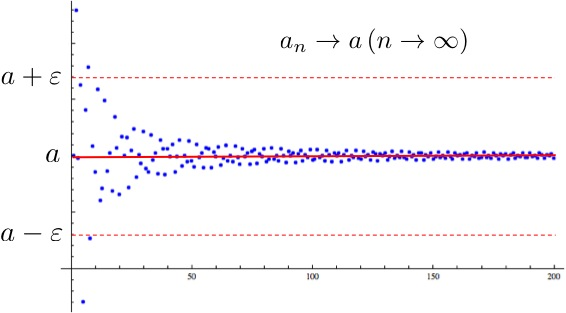
\includegraphics{./images/ch2/lim-en/en1.jpg}}\quad
	\resizebox{!}{3cm}{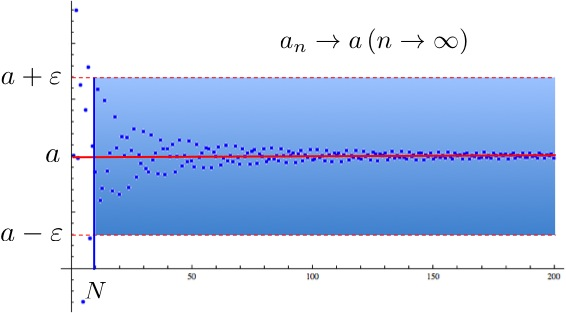
\includegraphics{./images/ch2/lim-en/en2.jpg}}
	
	\resizebox{!}{3cm}{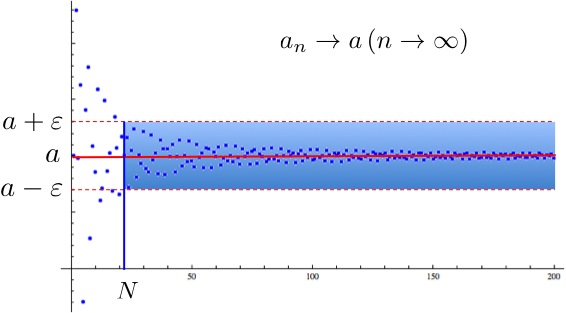
\includegraphics{./images/ch2/lim-en/en3.jpg}}\quad
	\resizebox{!}{3cm}{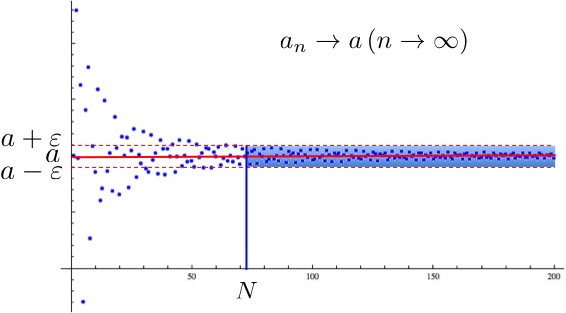
\includegraphics{./images/ch2/lim-en/en4.jpg}}
	
	\resizebox{!}{3cm}{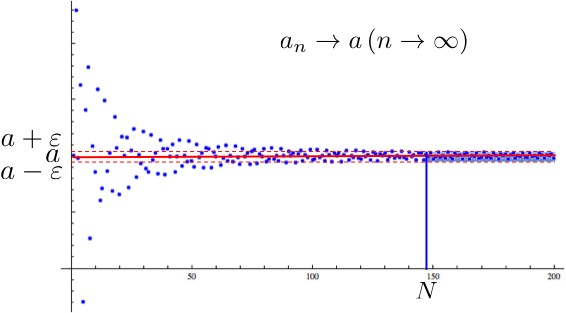
\includegraphics{./images/ch2/lim-en/en5.jpg}}
\end{center}

等价说法:

$$\lim_{n\to\infty}a_n=a\Leftrightarrow
\forall\e>0,\exists N\in\mathbb{Z}_+,\forall n>N,|a_n-a|<\e\eqno{(1)}$$

{\bf 讨论:}以下说法和$(1)$等价的是:

\begin{enumerate}
  \setlength{\itemindent}{1cm}
%   \item[(2)] $\forall\e>0$,$\exists N>0$,$\forall
%   n>N$,$|a_n-a|<\e$ \hfill{$\surd$}\\
%   \hfill(直接写$\exists N$即可)
  \item[(2)] $\forall\e>0$,$\exists N$,$\forall
  n>N$,$|a_n-a|\leq\e$ \hfill{$\surd$} 
  \item[(3)] $\exists N>0$,$\forall\e>0$,$\forall
  n>N$,$|a_n-a|<\e$ \hfill{$\times$} 
  \item[(4)] $\forall\e>0$,仅有有限多个$n$,使得$|a_n-a|\geq\e$
  \hfill{$\surd$} 
  \item[(5)] $\forall\e>0$,总有无穷多个$n$,使得$|a_n-a|<\e$
  \hfill{$\times$} 
  \item[(6)] $\forall\e>0$,要使$|a_n-a|<\e$,只须$n$充分大 \hfill{$\surd$}
  \item[(7)] $\forall\e>0,\exists N\in\mathbb{N}_+,\forall
  n>N,|a_n-a|<2\e$\hfill{$\surd$}
\end{enumerate}

{\bf 注:}

\begin{itemize}
  \setlength{\itemindent}{1cm}
  \item $a$是确定的数 ( {不能是$\pm\infty$}) 
  \item “$\forall\e>0$”应该理解为{“对任意小的$\e>0$”}
  \item $N$由$\{a_n\}$和$\e$共同决定, “存在$N$”可理解为{“存在充分大的$N(\e)$}”; 
   {如果$N$能够满足定义, 任意比$N$大的数都能够满足定义; 通常$\e$取得越小,
  $N$需要取得越大} \ps{$\{a_n\}$的收敛性与其任意多的有限项无关!!}
  \item 给定$C>0$,“$|a_n-a|<\e$” 可替换为{“$|a_n-a|<C\e$”}, 其中$C>0$为常数
\end{itemize}

{\bf 例:}证明:
$$\limn(-1)^n\df1{n^2}=0$$

{\bf 例:}证明:
$$\limn\left(\df n{n+1}\right)^2=1$$

{\bf 例:}证明:若$\limn a_n=a$,则$\limn|a_n|=|a|$

{\bf 例:}证明:若$|q|<1$,则$\{q^n\}$收敛。

{\bf 思考:}已知$|q|>1$时,$\{q^n\}$发散,请问该如何证明?

{\bf 注:}利用有界性,也可以证明发散。

\begin{shaded}
	{\bf 【极限定义的反面说法】}
	
	$$\limn a_n\neq a\Leftrightarrow\exists\e_0>0,\forall N>0,\exists
		n_0>N,|a_{n_0}-a|\geq\e_0$$
	
	{\bf 例:}证明:$\limn\df 1n\neq 1$
	
	{\bf P51,例5:}证明$\{(-1)^n\}$发散。 
	
	{\bf 注:}对比教材上的证明方法与用反面说法证明的区别。
	
	{\bf 思考:}数列发散可能有哪些不同的情形?(趋向无穷,或振荡)
	
\end{shaded}

\subsection{数列极限的基本性质}

\subsubsection{【唯一性】}

{\bf 定理2.1.1:}数列极限若存在,必唯一。\ps{唯一性的要求决定了当前的极限定义。
“记录重大技术突破的技术发展史其实就是一部人类社会发展的技术选择史”}

\begin{center}
	\resizebox{!}{4cm}{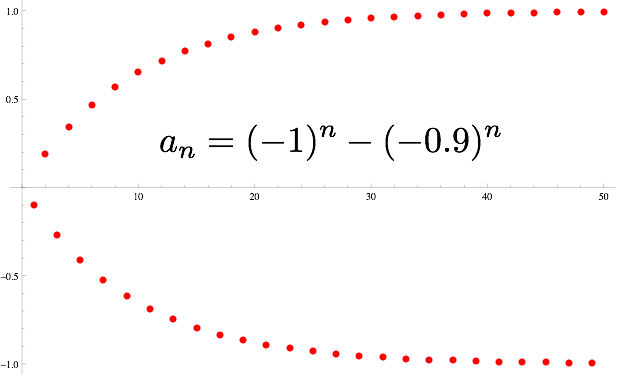
\includegraphics{./images/ch2/1-0.9n.jpg}}
\end{center}

{\bf 典型方法:}若对$\forall\e>0$,有$|a-b|<\e$,则$a=b$

\subsubsection{【有界性】}

{\bf 定理2.1.2:}数列$\{a_n\}$若收敛,则$\{a_n|n\in\mathbb{Z}_+\}$必有界。

\begin{center}
	\resizebox{!}{4cm}{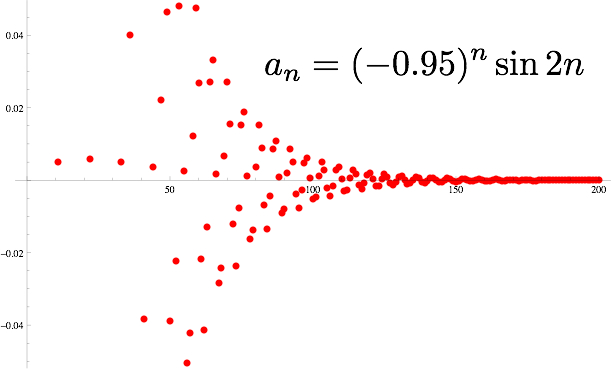
\includegraphics{./images/ch2/sin2nn.jpg}}
\end{center}

{\bf 典型方法:}利用$\e$的特定取值控制无穷的部分,剩余的有限集自然是有界的

{\bf 例:}讨论$\{\sqrt[n]{n!}\}$的敛散性。

{\bf hint:}注意到$\forall a>0$,当$n$充分大时,$n!>a^n$,故$\{\sqrt[n]{n!}\}$无界,
从而发散。

\subsubsection{【保号性】}

{\bf 定理2.1.3:}设$\lim\limits_{n\to\infty}a_n>0$,则$\exists N>0$,
		对$\forall n>N$,$a_n>0$
		
{{\bf 推论:}} 
\begin{enumerate}
  \setlength{\itemindent}{1cm}
  \item 设对$\forall n\in\mathbb{N}$,$a_n\geq
  0$, $\lim\limits_{n\to\infty}a_n=a$, 则$a\geq 0$ 
  \item 设$\lim\limits_{n\to\infty}a_n=a\ne
  0$, 则$\exists N$,当$n>N$时,$|a_n|>|a|/2$ 
  \item
  设$\lim\limits_{n\to\infty}a_n=a$, 且最多有有限个$a_n$小于零, 则$a\geq 0$
\end{enumerate}	

{\bf 注:}保号性的实质,是极限运算保持不等号的方向不变
$$a_n\geq b_n\,(n\in\mathbb{Z}_+)\Rightarrow\limn a_n\geq\limn b_n$$

\section{数列极限的性质与判敛}

\subsection{四则运算的性质}

{\bf 定理2.2.1:}\ps{强调:只对有限次的四则运算有效!!!}
设数列$\{a_n\},\{b_n\}$分别以$a,b(b\neq 0)$为极限,则
数列$\{a_n\pm b_n\},\{a_nb_n\},\left\{\df{a_n}{b_n}\right\}$均收敛,且
\begin{enumerate}
  \setlength{\itemindent}{1cm}
  \item $\limn(a_n\pm b_n)=a\pm b$
  \item $\limn a_nb_n=ab$
  \item $\limn\df{a_n}{b_n}=\df ab$
\end{enumerate}

{\bf 注:}极限运算和四则运算可以交换次序——前提是极限存在,且为有限次四则运算

{\bf 例:}
\begin{eqnarray*}
	1&=&\limn \underbrace{\left(\df 1n+\df 1n+\cdots+\df 1n\right)}_{n}\\
	&=&\underbrace{\limn\df1n+\limn\df1n+\cdots+\limn\df1n}_{n}\\
	&=&n\limn\df1n=0
\end{eqnarray*}
$n$落在了极限符号之外,显然错误!!

{\bf P58-例2:}计算极限
$$\limn\df{2n^6+3n^4-n+10}{n^6+n^4+1}$$

{\bf P58-例1:}设$\limn(a_n+b_n)=1$,$\limn(a_n-b_n)=3$,证明$\{a_n\},\{b_n\}$收敛,并求其值。

{\bf 例:}计算极限
$$\limn\df{\cos^n\theta-\sin^n\theta}{\cos^n\theta+\sin^n\theta}\quad
(0\leq\theta\leq\df{\pi}{2})$$

{\bf 定理2.2.1':}初等函数运算可以和极限运算交换次序。

{\bf 例:}设$a_n>0(n\in\mathbb{N})$,$\limn a_n=a$,证明:
$$\limn\sqrt{a_n}=\sqrt a$$

{\bf hint:} 若$a=0$,对$\e^2$,取$N$即可。

\subsection{子数列的收敛性}

{\bf 子数列:}

$$\{a_{n_k}\}:\,a_{n_1},a_{n_2},\ldots,a_{n_k},\ldots$$

{\bf 注:}$\{n_k\}$本质上是一个正整数构成的数列,
所以子数列可以视为两个数列的复合

{\bf 定理2.2.2:}数列收敛,当且仅当其任意子数列收敛,且极限相同。

即:对任意严格单调递增的正整数数列$\{n_k\}$,
$$\limn a_n=a\Leftrightarrow\lim_{k\to\infty}a_{n_k}=a$$
$\{a_{n_k}\}$收敛于$a$的定义: $\forall \e>0$, $\exists
{K}$, $\forall {k>K}$, 有 $$|a_{{{n_k}}}-a|<\e,$$
 记为\ps{强调$k$变化而不是$n$变化}
$$\lim\limits_{{k\to\infty}}a_{n_k}=a\quad \mbox{或}\quad a_{n_k}\to
a\;{(k\to\infty)}$$


{\bf 推论:}若某个数列存在不收敛的子列,或者存在两个极限不相同的子列,则该数列不收敛。

{\bf 例P60,例4:}证明数列$\left\{n^{(-1)^n}\right\}$发散。

{\bf 定理2.2.3}(拉链定理)数列$\{a_n\}$收敛,当且仅当$\{a_{2n}\}$
和$\{a_{2n-1}\}$收敛于相同的极限。

{\bf 推论:}数列$\{a_n\}$收敛,当且仅当$\{a_{3n}\}$,$\{a_{3n+1}\}$和
$\{a_{3n+2}\}$收敛于相同的极限。

{\bf 注:}更一般性的推广:如果选择的子列能够完全覆盖原数列,或最多不能覆盖原数列中
有限多个数,且这些子列均收敛于相同的极限,则原数列收敛。

\subsection{夹逼(迫敛)定理}

{\bf 定理2.2.4:}设对任意$n\in\mathbb{N}$,$x_n\le a_n\le y_n$,
且$\{x_n\},\{y_n\}$收敛于相同的极限$a$,则$\limn a_n=a$。

\begin{center}
	\resizebox{!}{5cm}{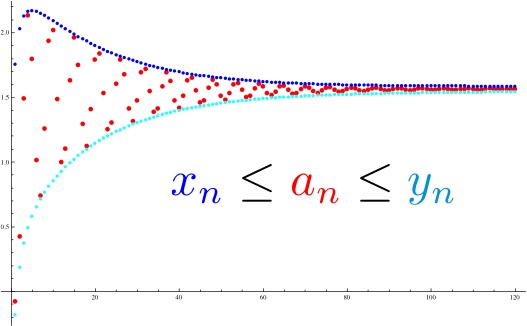
\includegraphics{./images/ch2/xay_n.jpg}}
\end{center}

{\bf P61,例5:}证明$\limn [(n+1)^k-{n}^k]=0$,其中$0<k<1$。

{\bf hint:}$n^k\left[\left(1+\df1n\right)^k-1\right]
<n^k\left(1+\df1n-1\right)=n^{k-1}\to 0\;(n\to\infty)$

{\bf P61,例6:}设$a>0$为常数,证明$\limn \sqrt[n]{a}=1$。

\subsection{单调有界原理}

{\bf 定理2.2.5:}单调有界的数列必收敛。\ps{只要数列从某一项开始单调即可!!!}

{\bf 【重要极限】}(P63-例7)
$$a_n=\left(1+\df{1}{n}\right)^n\to e\quad (n\to\infty)$$

{\bf 注:}需要掌握的重要性质
\begin{itemize}
  \setlength{\itemindent}{1cm}
  \item 数列$\left\{\left(1+\df 1n\right)^n\right\}$严格单调递增有上界
  \item 数列$\left\{\left(1+\df 1n\right)^{n+1}\right\}$严格单调递减有下界
  \item 显然,二者极限相同
\end{itemize}

\subsection{递推数列的判敛}

{\bf 例:}已知$a_1,a_2$为常数,数列$\{a_n\}$满足:
$$a_n=\df 12({a_{n-1}+a_{n-2}})\quad(n>2).$$
证明$\{a_n\}$收敛,并求其极限。

{\bf P65-例9:}设$a_1>0$,$a_{n+1}=\df 12\left(a_n+\df 1{a_n}\right)\,
(n=1,2,\ldots)$,证明$\{a_n\}$收敛,并求其极限。

{\bf 注:}
\begin{itemize}
  \setlength{\itemindent}{1cm}
  \item 递推式两边同时取极限,解方程求得极限的值,是最便利的计算递推数列极限的方法
  \item 若通过以上方法可以求出极限的值,通常只需证明数列单调有界即可
  \item 若该方法无法求得极限的值,则只能利用递推式推导数列通项,进而证明其收敛并计算极限
\end{itemize}

{\bf 例:}计算下列极限
\begin{enumerate}[(1)]
  \setlength{\itemindent}{1cm}
  \item $\limn\df{n^2}{a^n}\quad (a>1)$
  \item $\limn\df{n!}{n^n}$
  \item $\limn\underbrace{\sqrt{c+\sqrt{c+\ldots+\sqrt{c}}}}_{n\mbox{\small
		  个根号}}$
\end{enumerate}

{\bf }若极限存在,可由通项公式反推递推式,然后两边取极限,解方程求得极限值

\begin{shaded}

\subsection{特殊的极限计算方法}

{\bf Stolz定理:}

设数列$\{y_n\}$满足$\limn\df 1{y_n}=0$,且$\{y_n\}$至少从某一项开始保持严格单调递增,
则对任意数列$\{x_n\}$,若$\limn\df{x_n-x_{n-1}}{y_n-y_{n-1}}$存在,则必有
$$\limn\df{x_n}{y_n}=\limn\df{x_n-x_{n-1}}{y_n-y_{n-1}}$$

{\bf 注:}Stolz定理主要用于计算"$\df{\infty}{\infty}$型"的极限

{\bf 推论:}若数列$\{a_n\}$收敛,则
$$\limn\df{a_1+a_2+\ldots+a_n}{n}=\limn a_n$$

{\bf 例:}计算以下极限
\begin{enumerate}[(1)]
  \setlength{\itemindent}{1cm}
  \item $\limn\df{1+\sqrt 2+\sqrt[3]{3}+\ldots+\sqrt[n]{n}}{n}$ 
  \item $\limn\df{1^k+2^k+\ldots+n^k}{n^{k+1}},\quad(k\in\mathbb{N})$ 
  \item $\limn\left(\df{1^k+2^k+\ldots+n^k}{n^{k}}-\df
  n{k+1}\right),\quad(k\in\mathbb{N})$\\
  {\bf 提示:}(3)
  \begin{eqnarray*}
  	\mbox{原式}&=&\limn\df{(k+1)(1^k+2^k+\cdots+n^k)-n^{k+1}}{n^k(k+1)}\\
  	&=&\limn\df{(k+1)(n+1)^k-[(n+1)^{k+1}-n^{k+1}]}{(k+1)[(n+1)^k-n^k]}\\
  	&=&\limn\df{(k+1)[n^k+kn^{k-1}+P_{k-2}^{(1)}(n)]
  	-\left[(n+1)^k+(n+1)^{k-1}n+\cdots+n^k\right]}{(k+1)
  	\left[(n+1)^{k-1}+(n+1)^{k-2}n+\cdots+n^{k-1}\right]}\\
  	&=&\limn\df{(k+1)[n^k+kn^{k-1}+P_{k-2}^{(1)}(n)]-(k+1)n^k
  	-\df{k(k+1)}2n^{k-1}-P_{k-2}^{(2)}(n)}
  	{(k+1)\left[\df{k(k+1)}{2}n^{k-1}+P_{k-2}^{(3)}(n)\right]}\\
  	&=&\df12
  \end{eqnarray*}
\end{enumerate}

\end{shaded}

\section{数值级数}

{\bf 级数(无穷和):}无穷多个数按照一定次序求和
$$\sum\limits_{k=1}^{\infty}a_k
=\lim_{n\to\infty}\left(\sum_{k=1}^na_k\right)$$  
其中$a_k\in\mathbb{R}\,(k\in\mathbb{N})$。

\begin{itemize}
  \item {\bf 部分和(数列):}$S_n=\sum\limits_{k=1}^na_k$
  \item {\bf 级数收敛}$\Leftrightarrow\{S_n\}$收敛
\end{itemize}

{\bf 例:}判断下列级数的收敛性
\begin{enumerate}[(1)]
  \setlength{\itemindent}{1cm}
  \item $\sumn q^n\quad (q>0)$ (\ldots\ldots 几何级数) 
  \item $\sumn\df{1}{n(n+1)}$ 
  \item $\sumn\df 1n$ (\ldots\ldots 调和级数) 
% 		  \item $\sumn\df 1n^2$
  \item $\sumn (-1)^n$
\end{enumerate}

\subsection{收敛级数的性质}

\begin{enumerate}[{\bf 【性质1】}]
  \item {\bf P74-定理2.3.1}(级数收敛的必要条件) 
  $$\sumn a_n\mbox{收敛}\Rightarrow\limn a_n=0$$
  \item $\sumn
  a_n$收敛$\Leftrightarrow\sum\limits_{n=k}^{\infty}a_n$收敛$(k\in\mathbb{N})$
  \ps{讨论收敛性时只需考虑部分和的后一部分,因为数列的收敛性与其前任意项无关}
  \item {\bf P73-例2:}$\{a_n\}$收敛$\Leftrightarrow\sumn(a_{n+1}-a_n)$收敛
  \item {\bf P75-定理2.3.2-3:}线性运算不改变级数的敛散性  
  \item {\bf P75-定理2.3.4:}增加、减少或改变级数中的有限项不影响其敛散性  
  \begin{itemize}
    \item {{增减或改变数列中的有限项不改变其敛散性}} 
  \end{itemize}
  \item {\bf P75-定理2.3.5:}若$\sumn a_n$收敛,不改变求和顺序,
  任意合并其中的项,所得新的级数仍收敛 
  \begin{itemize}
    \item {\bf 推论:}合并收敛级数中的相邻项,所得级数仍收敛 
    \item {{对发散级数,该性质不成立}} 
    \item {{改变求和次序,可能改变级数的收敛和}},例:$\sumn\df{(-1)^n}n$
  \end{itemize}
\end{enumerate}

{\bf 例:}判断以下级数的敛散性;若收敛,求其和

\begin{enumerate}[(1)]
  \setlength{\itemindent}{1cm}
  \item $\sumn\ln\left(1+\df 1n\right)$
  \item
  $\sumn\left[\prod\limits_{k=0}^p(\alpha+n+k)\right]^{-1},\;(p\in\mathbb{N})$
  \item $\sumn\df{x^{2^{n-1}}}{1-x^{2n}}$
  \item $\sumn\df{1}{\sqrt n}$
\end{enumerate}

\section{同号级数的收敛性}

\subsection{同号级数收敛的充要条件}

{\bf 定理2.4.1:}正项级数收敛,当且仅当其部分和数列有界。

{\bf P80,例1:}证明$\sumn\df1{n!}$收敛。

\subsection{比较判别法}

{\bf 定理2.4.2}(比较判别法的不等式形式)若对充分大的$n$,总有$0\leq a_n\leq b_n$,则
\begin{enumerate}
  \setlength{\itemindent}{1cm}
  \item 若$\sumn b_n$收敛,则$\sumn a_n$收敛
  \item 若$\sumn a_n$发散,则$\sumn b_n$发散
\end{enumerate}

{\bf P82-例3:}证明:\ps{p-级数}
\begin{enumerate}[(1)]
  \setlength{\itemindent}{1cm}
  \item[(1)] $p>1$时,$\sumn\df1{n^p}$收敛;
  \item[(2)] $0<p\leq 1$时,$\sumn\df1{n^p}$发散。
\end{enumerate}

{\bf 【hint】:}(2),$p=1$时,显然发散。又因为
$$0<\df 1n<\df 1{n^p},\quad (0<p<1),$$
已知调和级数发散,故p-级数发散;

(1)由以下推导可知$p>1$时,p-级数的部分和数列有界
\begin{eqnarray*}
	S_{(2^k)^p}&=&1+\df 1{2^p}+\underbrace{\left(\df1{3^p}+\df1{(2^2)^p}\right)}_2
				+\underbrace{\left(\df1{5^p}+\ldots+\df1{(2^3)^p}\right)}_{2^2}+\ldots\\
				&&+\underbrace{\left[\df1{(2^{k-1}+1)^p}+\ldots+\df1{(2^k)^p}\right]}_{2^{k-1}}\\
			  &\leq &1+\df 1{2^p}+2\cdot\df1{2^p}+2^2\cdot\df1{(2^2)^p}
			    +\ldots+2^{k-1}\cdot\df1{(2^{k-1})^p}\\
			  &=&1+\df 1{2^p}+\left[\df1{2^{p-1}}+\left(\df1{2^{p-1}}\right)^2+
			    \ldots+\left(\df1{2^{p-1}}\right)^{k-1}\right]\\
			  &=&1+\df 1{2^p}+\df1{2^{p-1}}\df{1-\left(\df1{2^{p-1}}\right)
			    ^{k-1}}{1-\df1{2^{p-1}}}<1+\df 1{2^p}+\df1{2^{p-1}-1}
\end{eqnarray*}

{\bf 例:}讨论下列级数的敛散性
\begin{enumerate}[(1)]
  \setlength{\itemindent}{1cm}
  \item[(1)] $\sumn\df{1}{3^{\ln n}}$
  \hfill({[hint]:$a^{\ln b}=b^{\ln a},\;(a,b>0)$})
  \item[(2)] $\sum\limits_{n=2}^{\infty}\df 1{(\ln n)^{\ln n}}$
  \item[(3)] $\sum\limits_{n=3}^{\infty}\df 1{(\ln n)^{\ln\ln n}}$
  
  ([hint]: $\sum\limits_{n=3}^{\infty}\df 1{(\ln n)^{\ln\ln n}}=
  \sum\limits_{n=3}^{\infty}\df 1{e^{(\ln\ln
  n)^2}}>\sum\limits_{n=3}^{\infty}\df 1n,e.g. (\ln\ln n)^2<\ln n,e.g. \ln
  n<\sqrt{n}$)
\end{enumerate}

{\bf P82-例4:}设$a_n\leq c_n\leq b_n\;(n\in\mathbb{N})$,$\sumn a_n,\sumn b_n$均收敛,
则$\sumn c_n$收敛。
\begin{itemize}
  \setlength{\itemindent}{1cm}
  \item 类似于数列收敛的“夹逼定理”
  \item 不要求必须是正项级数
\end{itemize}

{\bf 推论}(P93-定理2.5.2)若级数$\sumn|a_n|$收敛,则$\sumn a_n$也收敛。

{\bf 定理2.4.3}(比较判别法的极限形式)

已知$a_n,b_n$均非负$(n\in\mathbb{Z}_+)$,且$\limn\df{a_n}{b_n}=l$,则 
\begin{enumerate}
  \setlength{\itemindent}{1cm}
  \item 若$0<l<+\infty$,$\sumn a_n,\sumn b_n$同敛散 
  \item 若$l=0$,$\sumn b_n$收敛$\Rightarrow\sumn a_n$收敛 
  \item 若$l=+\infty$,$\sumn a_n$收敛$\Rightarrow\sumn b_n$收敛
\end{enumerate}

{\bf P83-例5-6:}判断以下级数的收敛性
\begin{enumerate}[(1)]
  \setlength{\itemindent}{1cm}
  \item $\sumn\df 1{2^n}\df{n^2+1}{2n^2-1}$ 
  \item $\sumn\df{n+1}{n^k+2}\quad (k=1,2,\ldots)$ 
  \item $\sumn\df{1}{n\sqrt[n]{n}}$ 
  \item $\sumn\df{1}{1+x^n}\quad(x>0)$
\end{enumerate}

{\bf 推论}(p-判别法)
设$a_n\geq 0\;(n=1,2,\ldots)$,则 
\begin{enumerate}
  \setlength{\itemindent}{1cm}
  \item 若存在$p>1$,使得$\limn n^pa_n$存在,则$\sumn a_n$收敛 
  \item 若$0<p\leq 1$,使得$\limn n^pa_n>0$,则$\sumn a_n$发散
\end{enumerate}

{\bf 例:}判断以下级数的收敛性
\begin{enumerate}[(1)]
  \setlength{\itemindent}{1cm}
  \item $\sumn\df{\arctan n}{n^{3/2}}$
  \item $\sumn\df{\ln n}{n^{5/4}}$\ps{任何正幂次函数的增长速度最终都比任意对数函数快}
\end{enumerate}

{\bf 推论:}$\sumn a_n$、$\sumn b_n$均为正项级数,若对充分大的$n$,总有
$$\df{a_{n+1}}{a_n}\leq\df{b_{n+1}}{b_n},$$
则若$\sumn b_n$收敛,$\sumn a_n$收敛。

{\bf 【hint】:}
$$a_{n+1}\leq\df{a_1}{b_1}b_{n+1}$$

{\bf 例:}讨论级数$\sumn\df{n^n}{t^nn!}$的敛散性。

{\bf 【hint】:}
$$\df{a_{n+1}}{a_n}=\df{\left(1+\df1n\right)^n}{t}\to\df et$$

{\bf 课后思考}(2012年全国大学生数学竞赛)
$\sumn a_n$和$\sumn b_n$均为正项级数,证明:
\begin{enumerate}
  \setlength{\itemindent}{1cm}
  \item 若$\limn\left(\df{a_n}{a_{n+1}b_n}-\df 1{b_{n+1}}\right)>0$,
  且$\sumn b_n$收敛,则$\sumn a_n$收敛;\ps{是否一定要假设$\sumn b_n$收敛?}
  \item 若$\limn\left(\df{a_n}{a_{n+1}b_n}-\df 1{b_{n+1}}\right)<0$,
  且$\sumn b_n$发散,则$\sumn a_n$发散。
\end{enumerate}

{\bf 牢记:比较判别法仅对同号级数有效!!!}

\subsection{比值判别法}

{\bf 定理2.4.4}(d'Alembert判别法)
设$a_n\geq 0(n=1,2,\ldots)$,$\limn\df{a_{n+1}}{a_n}=q$,则
\ps{极限形式} 
\begin{enumerate}
  \setlength{\itemindent}{1cm}
  \item $0\leq q<1\Rightarrow\sumn a_n$收敛 
  \item $q>1\Rightarrow\sumn a_n$发散
\end{enumerate}

{\bf 注:}$q=1$时,级数的敛散性不确定,例如:$\sumn\df 1n$和$\sumn\df 1{n^2}$

{\bf P83-85-例5-7:}判断下列级数的收敛性
\begin{enumerate} [(1)]
  \setlength{\itemindent}{1cm}
  \item $\sumn\df 1{2^n}\df{n^2+1}{2n^2-1}$ 
  \item $\sumn\df{n^2}{2^n}$ 
  \item $\sumn\df{(2n)!}{(n!)^2}$
  \item $\sumn n!\left(\df{x}{n}\right)^n\quad (x>0)$
\end{enumerate}

{\bf 定理2.4.4‘}(习题2.4-11:比值判别法的不等式形式)
设$a_n\geq 0\,(n=1,2,\ldots)$,则 
\begin{enumerate}
  \setlength{\itemindent}{1cm}
  \item 若$n$充分大时,有$\df{a_{n+1}}{a_n}\leq r<1$,则$\sumn a_n$收敛 
  \item 若$n$充分大时,有$\df{a_{n+1}}{a_n}\geq 1$,则$\sumn a_n$发散 
\end{enumerate}

{\bf 思考:}为什么以上第一个判定条件中要求$r<1$?

{\bf P86-例8:}判断以下级数的收敛性
$$\sumn\df{2+(-1)^n}{n^2}$$

\subsection{根值判别法}

{\bf 定理2.4.5}(Cauchy判别法)\ps{极限形式}
设$a_n\geq 0(n=1,2,\ldots)$,$\limn\sqrt[n]{a_n}=q$,则
\begin{enumerate}
  \setlength{\itemindent}{1cm}
  \item $0\leq q<1\Rightarrow\sumn a_n$收敛
  \item $q>1\Rightarrow\sumn a_n$发散
\end{enumerate}

{\bf 注:}
\begin{itemize}
  \setlength{\itemindent}{1cm}
  \item 和比值法类似,$q=1$时,无法判定级数的敛散性
  \item
  但是,可以证明:若$\limn\df{a_{n+1}}{a_n}=q$,则必有$\limn\sqrt[n]{a_n}=q$,请问:
  这意味着比值和根植法哪一个的适用范围更广?(答:根植)
\end{itemize}

{\bf P86-例8:}判断下列级数的收敛性
\begin{enumerate} [(1)]
  \setlength{\itemindent}{1cm}
  \item $\sumn\df{2+(-1)^n}{5^n}$
  \item $\sumn\df{n^2}{\left(2+\df 1n\right)^n}$
  \item $\df 12+\df 1{3^2}+\df 1{2^3}+\df 1{3^4}+\df 1{2^5}+\df 1{3^6}+\ldots$
\end{enumerate}

{\bf 思考:}根植判别法的不等式形式该如何表述?

\begin{shaded}

\subsection{Raabe判别法*}

{\bf Raabe判别法:}设$a_n\geq 0\,(n=1,2,\ldots)$,且
$$\limn n\left(\df{a_n}{a_{n+1}}-1\right)=r,$$
则当$r>1$时,$\sumn a_n$收敛;$r\leq 1$时,$\sumn a_n$发散。	

{\bf 例:}判断以下级数的敛散性
\begin{enumerate}[(1)]
  \setlength{\itemindent}{1cm}
  \item $\sumn\df{(2n-1)!!}{(2n)!!}\df 1{2n+1}$
  \item $\sumn\df{n!}{(x+1)\ldots(x+n)}\;(x>0)$
\end{enumerate}

{\bf 【hint】:}(1)
$$R_n=n\left[\df{(2n+2)(2n+3)}{(2n+1)(2n+1)}-1\right]
=\df{n(6n+5)}{(2n+1)^2}\to\df32>1\;(n\to\infty)$$
(2)
$$R_n=n\left[\df{n+x}{n+1}-1\right]=\df{n(x-1)}{n+1}$$

{\bf 不等式形式:}设$a_n\geq 0\,(n=1,2,\ldots)$,定义
$$R_n=n\left(\df{a_n}{a_{n+1}}-1\right),$$
若存在$r>1$,当$n$充分大时,总有$R_n\geq r$,则$\sumn a_n$收敛;
若当$n$充分大时,总有$R_n\leq 1$,则$\sumn a_n$发散。

{\bf 例:}判断以下级数的敛散性
$$\sumn\df{\sqrt{n!}}{(2+\sqrt 1)(2+\sqrt 2)\ldots(2+\sqrt n)}$$

{\bf 【hint】:}记$a_n=\df{\sqrt{n!}}{(2+\sqrt 1)(2+\sqrt 2)\ldots(2+\sqrt n)}$,
从而
$$n\left(\df{a_n}{a_{n+1}}-1\right)=\df{2n}{\sqrt{n+1}}\to\infty\;(n\to\infty)$$
从而易知该级数发散。

\end{shaded}

\section{变号级数收敛的判定方法}

\subsection{交错级数的收敛性}

{\bf 交错级数:}相邻各项符号相反,设$a_n\geq 0,(n\in\mathbb{Z}_+)$
$$\sumn(-1)^na_n$$

{\bf 定理2.5.1}(Leibniz判别法)若数列$\{a_n\}$单调趋于$0$,则交错级数$\sumn (-1)^na_n$收敛,且
其和的绝对值不超过$|a_1|$。

{\bf 注:}Leibniz判别法只是一个充分条件,常见的错误,将其作为必要条件使用!!!

{\bf 例:}判断下列级数的敛散性
\begin{enumerate} [(1)]
  \setlength{\itemindent}{1cm}
  \item $\sumn(-1)^{n-1}\df{2^nn!}{n^n}$ 
  \item $\sumn(-1)^n\df{\sqrt{n}}{n+100}$ 
  \item $\sumn\sin\left(\pi\sqrt{n^2+k^2}\right)$
\end{enumerate}

\subsection{绝对收敛与条件收敛}

{\bf 定理2.5.2:}若$\sumn |a_n|$收敛,则$\sumn a_n$收敛;反之不然。

{\bf 定理2.5.3-2.5.4}(绝对收敛级数的性质)

\begin{itemize}
  \setlength{\itemindent}{1cm}
  \item {\bf 绝对收敛:}$\sumn |a_n|$收敛\ps{这样已经隐含了$\sumn a_n$收敛}
  \item {\bf 条件收敛:}$\sumn |a_n|$发散,但$\sumn a_n$收敛
\end{itemize}

\begin{enumerate}[(1)]
  \setlength{\itemindent}{1cm}
  \item {\bf 交换律:}绝对收敛级数求和项任意交换次序和不变\ps{强调:交换次序意味着新的级数}
  \item {\bf 级数的Cauchy乘积:}设$\sumn a_n,\sumn
	  b_n$绝对收敛,则$\sum\limits_{i,j=1}^na_ib_j$绝对收敛,且
	  $$\sum\limits_{i,j=1}^{\infty}a_ib_j=\sumn a_n\sumn b_n$$
\end{enumerate}

\begin{shaded}

\subsection{特殊判别法}

{\bf Dirichlet判别法:}若数列$\{a_n\}$单调趋于$0$,$\sumn b_n$
  的部分和有界,则$\sumn a_nb_n$收敛。
  
{\bf 例:}判断以下级数的敛散性
$$\sumn\df{\sin nx}n$$

{\bf Abel判别法:}若数列$\{a_n\}$单调有界,$\sumn b_n$收敛,则$\sumn a_nb_n$收敛。

{\bf 例:}判断以下级数的敛散性

$$\sumn(-1)^n\left(1+\df 1n\right)^n\df{1}{\sqrt n}$$ 

\subsection{条件收敛的有趣性质}

{\bf Riemann定理:}若级数$\sumn a_n$条件收敛,则对任意给定的数$A$,都可以通过对该级数的
重新排列,使得新的级数以$A$为其和。

\begin{itemize}
  \item 对条件收敛的级数进行重排可能改变其和
  \item 重排后的级数可能发散
\end{itemize}

\end{shaded}

\begin{center}
	\resizebox{!}{6.8cm}{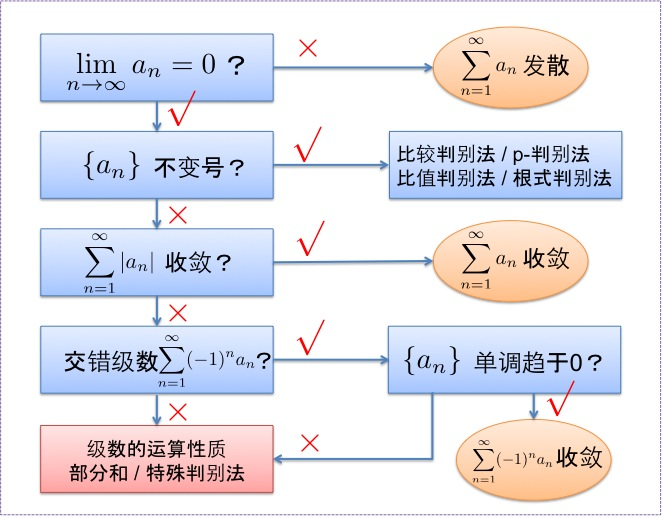
\includegraphics{./images/ch2/seriesCre/010.jpg}}
\end{center}

{\bf 例:}判断正误:
\begin{enumerate}[(1)]
  \setlength{\itemindent}{1cm}
  \item 若$a_n>0(n=1,2,\ldots)$,则\\
  \centerline{$a_1-a_1+a_2-a_2+a_3-a_3+\ldots $}
  收敛 \hfill ({$\times$})
  \item 若以上$\limn a_n=0$,则以上级数收敛 \hfill
  ({$\surd$})
  \item $\sumn a_n$收敛,$\limn b_n=1\Rightarrow\sumn a_nb_n$收敛
  \hfill ({$\times$})
  \item $\sumn a_n$部分和有界,$\limn b_n=0\Rightarrow\sumn a_nb_n$收敛
  \hfill ({$\times$})
  \item 若$\limn\df{a_n}{b_n}=1$,则若$\sumn a_n$绝对收敛,$\sumn b_n$必收敛 \hfill
  ({$\surd$})
  \item $\sumn a_n,\sumn b_n$绝对收敛$\Rightarrow\sumn (a_n+b_n)$绝对收敛 \hfill
  ({$\surd$})
  \item $\sumn a_n,\sumn b_n$条件收敛$\Rightarrow\sumn (a_n+b_n)$条件收敛 \hfill
  ({$\times$})
  \item 若$\sumn a_n^2$收敛,则$\sumn a_n^3$收敛 \hfill
  ({$\surd$})
\end{enumerate}

{\bf 例:}判断下列级数的敛散性
\begin{enumerate}[(1)]
  \setlength{\itemindent}{1cm}
  \item $\sumn\df{2^nn!}{n^n}$
  \item $\df 1{a+b}+\df 1{2a+b}+\df 1{3a+b}+\ldots\quad (a>0,b>0)$
  \item $\sumn\df{1!+2!+\ldots+n!}{n!}$
  \item $\sumn\left[\df 1n-\ln\left(1+\df 1n\right)\right]$
  \item $\sumn\df{\sqrt{n!}}{(2+\sqrt 1)(2+\sqrt 2)\ldots(2+\sqrt n)}$
  \item $\sumn\df{\sqrt{n+1}-\sqrt{n}}{n^p}\quad(p>0)$
  \item $\sumn\df{n^{n+\frac 1{\,n\,}}}{\left(n+\df 1n\right)^n}$
  \item $\sumn n!\left(\df{x}{n}\right)^n\quad (x>0)$
  \item $\sumn\df {a_n}{(1+a_1)(1+a_2)\ldots(1+a_n)}\quad(a_n\geq
	  0,n\in\mathbb{N})$
  \item $\sumn\df{n^{n+\frac 1{\,n\,}}}{\left(n+\df 1n\right)^n}$
\end{enumerate}

\newpage

\section*{课后作业}

\begin{itemize}
  \item 习题2.1:2,6(1,3),7,9
  \item 已知数列$\{a_n\}$单调递增,它的一个子列$\{a_{n_k}\}$收敛于$a$,
  证明:$\limn a_n=a$。
  \item 证明:$\sqrt[n]n\to 1\,(n\to\infty)$。
  \item 习题2.2:1(4,6),2(2,3),3,7,9,11
  \item 习题2.3:4,5,6
  \item 写出根植判别法的不等式形式,并证明。
  \item 习题2.4:1(2-4),3(3-8),5(2,4),6(1-3),8,9
  \item 习题2.5:2(1,3,6,7,8),3,7,8
\end{itemize}

{\bf 【课堂练习与思考题】}

\begin{itemize}
  \item 习题2.2:6,8,10,12,18
  \item 设$0<a_1<2$,且$(2-a_n)a_{n+1}=1\,(n\in\mathbb{N})$,
  	证明$\{a_n\}$收敛,求其极限。
  \item 设$x_1=\df 12$,$x_{n+1}=x_n^2+x_n\,(n\in\mathbb{N})$,求
	$$\limn\left(\df 1{x_1+1}+\df 1{x_2+1}+\ldots+\df
	1{x_n+1}\right)$$
  \item 已知$0<x<1$,数列$\{a_n\}$定义如下:
	$$a_1=\df x2,\;a_n=\df x2-\df{a_{n-1}^2}2.$$
	证明$\{a_n\}$收敛,并求其极限。
  \item 习题2.3:7,8 
  \item 习题2.4:10-15,17
  \item 习题2.5:4,6,10,13
\end{itemize}

\end{document}
